%%%%%%%%%%%%%%%%%%%%%%%%%%%%%%%%%%%%%%%%%%%%%%%%%%%
%% P3: Phenomenology of Particle Physics                         
%%
%% Author:  André Rubbia                   		 
%%
%% Figure 2.22 The photon cross-section on lead (Pb, $Z=82$). 
%%
%% This work is licensed under the Creative Commons Attribution 4.0 International License. 
%% To view a copy of this license, visit http://creativecommons.org/licenses/by/4.0/ or 
%% send a letter to Creative Commons, PO Box 1866, Mountain View, CA 94042, USA.
%%
%% Data taken Data taken from the Physical Measurement Laboratory of the National Institute of Standards and Technology (NIST) 
%% (http://physics.nist.gov/)
%%
%%%%%%%%%%%%%%%%%%%%%%%%%%%%%%%%%%%%%%%%%%%%%%%%%%%

\documentclass[a4paper,10pt]{article}

\usepackage[T1]{fontenc}
\usepackage[utf8]{inputenc}
\usepackage{lmodern}
\usepackage[labelfont=bf]{caption}
\usepackage{upgreek}
\usepackage{amssymb}
\usepackage{amsmath}

\usepackage{tikz}
\usepackage{pgfplots}
\pgfplotsset{compat=1.17}
\usepgfplotslibrary{ternary}
\usepgfplotslibrary{fillbetween}
\usepgfplotslibrary{external}


\def\d{\mathrm{d}}

\begin{document}

%%%%%%%%%%%%%%%   FIGURE  %%%%%%%%%%%%%%%%%%%%%%%%%%%%%%
\begin{figure}[htb]
\begin{center}
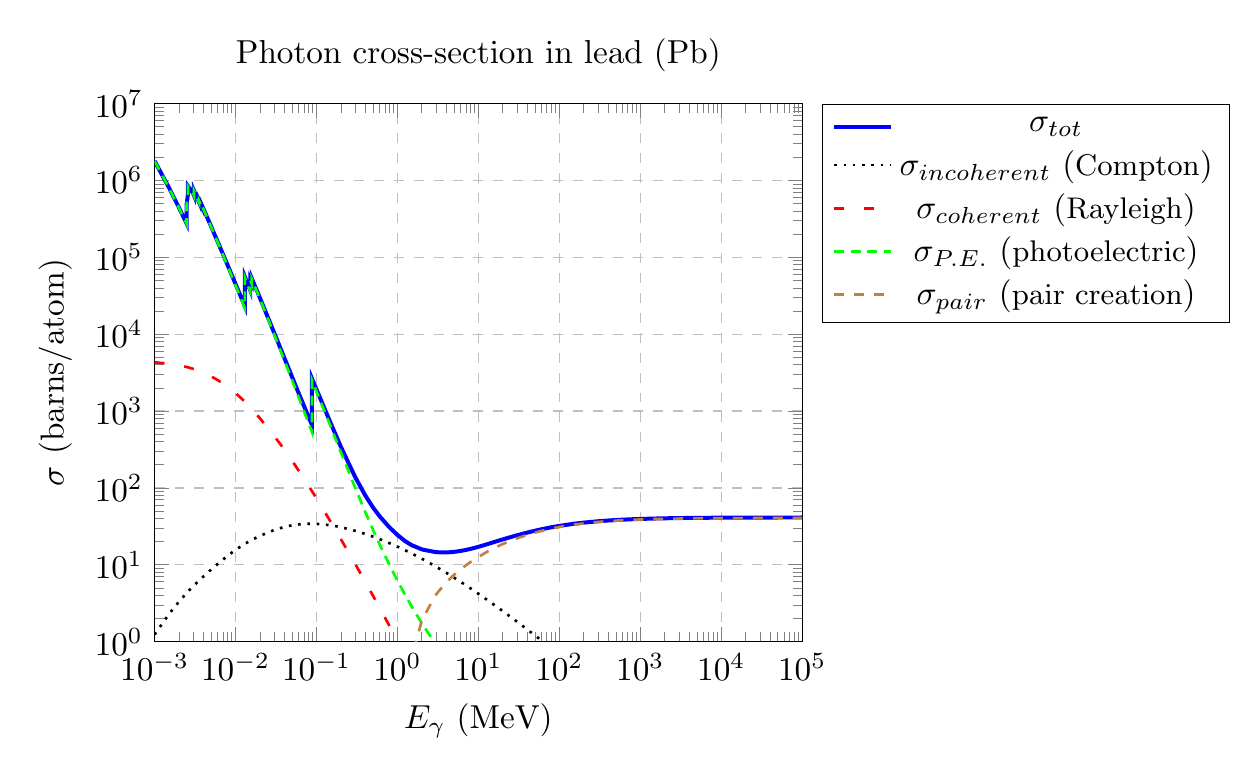
\begin{tikzpicture}[scale=1.2]
\begin{loglogaxis}[
    title={Photon cross-section in lead (Pb)},
    xlabel={$E_\gamma$ (MeV)},
    ylabel={$\sigma$ (barns/atom)},
    xmin=1e-3, xmax=1e5,
    ymin=1, ymax=1e7,
%    xtick={0,20,40,60,80,100,120,140,160},
%    ytick={1e0,1e1,1e2,1e3,1e4,1e5,1e6,1e7},
    legend pos=outer north east,
    ymajorgrids=true,
    xmajorgrids=true,
    grid style=dashed,
]
%% total
\addplot[
    color=blue, very thick,
    ]
    coordinates {
(0.001,1.792e+06)
(0.0015,810700)
(0.002,442200)
(0.002484,275500)
(0.002484,480200)
(0.002534,566700)
(0.002586,668700)
(0.002586,842900)
(0.003,676000)
(0.003066,638900)
(0.003066,738400)
(0.003301,616500)
(0.003554,514600)
(0.003554,545200)
(0.003699,495900)
(0.003851,451100)
(0.003851,470600)
(0.004,430500)
(0.005,251300)
(0.006,160700)
(0.008,78680)
(0.01,44950)
(0.01304,23050)
(0.01304,55770)
(0.015,38390)
(0.0152,37080)
(0.0152,51100)
(0.01553,48600)
(0.01586,46230)
(0.01586,53270)
(0.02,29720)
(0.03,10430)
(0.04,4941)
(0.05,2767)
(0.06,1727)
(0.08,832.4)
(0.088,657.1)
(0.088,2644)
(0.1,1909)
(0.15,693.1)
(0.2,343.6)
(0.3,138.7)
(0.4,79.92)
(0.5,55.51)
(0.6,42.92)
(0.8,30.52)
(1,24.43)
(1.022,23.95)
(1.25,20.21)
(1.5,17.97)
(2,15.85)
(2.044,15.75)
(3,14.57)
(4,14.44)
(5,14.7)
(6,15.11)
(7,15.58)
(8,16.08)
(9,16.59)
(10,17.11)
(11,17.61)
(12,18.1)
(13,18.57)
(14,19.03)
(15,19.47)
(16,19.88)
(18,20.65)
(20,21.35)
(22,22)
(24,22.6)
(26,23.16)
(28,23.68)
(30,24.16)
(40,26.18)
(50,27.72)
(60,28.93)
(80,30.74)
(100,32.03)
(150,34.09)
(200,35.33)
(300,36.78)
(400,37.62)
(500,38.16)
(600,38.56)
(800,39.09)
(1000,39.42)
(1500,39.92)
(2000,40.19)
(3000,40.48)
(4000,40.64)
(5000,40.73)
(6000,40.8)
(8000,40.89)
(10000,40.95)
(15000,41.03)
(20000,41.08)
(30000,41.12)
(40000,41.14)
(50000,41.16)
(60000,41.17)
(80000,41.17)
(100000,41.18)
  };

% incoherent
\addplot[
    color=black, dotted, thick,
    ]
    coordinates {
(0.001,1.234)
(0.0015,2.271)
(0.002,3.31)
(0.002484,4.266)
(0.002484,4.266)
(0.002534,4.364)
(0.002586,4.463)
(0.002586,4.463)
(0.003,5.246)
(0.003066,5.369)
(0.003066,5.369)
(0.003301,5.793)
(0.003554,6.238)
(0.003554,6.238)
(0.003699,6.491)
(0.003851,6.753)
(0.003851,6.753)
(0.004,7.009)
(0.005,8.655)
(0.006,10.22)
(0.008,13.1)
(0.01,15.62)
(0.01304,18.7)
(0.01304,18.7)
(0.015,20.37)
(0.0152,20.52)
(0.0152,20.52)
(0.01553,20.77)
(0.01586,21.03)
(0.01586,21.03)
(0.02,23.73)
(0.03,28.31)
(0.04,31.03)
(0.05,32.61)
(0.06,33.49)
(0.08,34.14)
(0.088,34.16)
(0.088,34.16)
(0.1,34.04)
(0.15,32.63)
(0.2,30.85)
(0.3,27.65)
(0.4,25.15)
(0.5,23.17)
(0.6,21.55)
(0.8,19.05)
(1,17.18)
(1.022,17.01)
(1.25,15.4)
(1.5,14.02)
(2,11.98)
(2.044,11.84)
(3,9.44)
(4,7.879)
(5,6.806)
(6,6.017)
(7,5.409)
(8,4.923)
(9,4.526)
(10,4.193)
(11,3.911)
(12,3.668)
(13,3.456)
(14,3.27)
(15,3.104)
(16,2.956)
(18,2.702)
(20,2.492)
(22,2.314)
(24,2.163)
(26,2.031)
(28,1.916)
(30,1.814)
(40,1.441)
(50,1.203)
(60,1.037)
(80,0.8176)
(100,0.6786)
(150,0.4833)
(200,0.3789)
(300,0.2686)
(400,0.2103)
(500,0.1741)
(600,0.1491)
(800,0.1164)
(1000,0.09579)
(1500,0.0669)
(2000,0.05178)
(3000,0.036)
(4000,0.02779)
(5000,0.02272)
(6000,0.01927)
(8000,0.01484)
(10000,0.01212)
(15000,0.008376)
(20000,0.00644)
(30000,0.004441)
(40000,0.003409)
(50000,0.002776)
(60000,0.002347)
(80000,0.0018)
(100000,0.001464)
};

% incoherent
\addplot[
    color=red, loosely dashed, thick,
    ]
    coordinates {
(0.001,4304)
(0.0015,4132)
(0.002,3935)
(0.002484,3742)
(0.002484,3742)
(0.002534,3722)
(0.002586,3701)
(0.002586,3701)
(0.003,3533)
(0.003066,3507)
(0.003066,3507)
(0.003301,3416)
(0.003554,3321)
(0.003554,3321)
(0.003699,3267)
(0.003851,3212)
(0.003851,3212)
(0.004,3158)
(0.005,2824)
(0.006,2533)
(0.008,2065)
(0.01,1714)
(0.01304,1325)
(0.01304,1325)
(0.015,1138)
(0.0152,1121)
(0.0152,1121)
(0.01553,1094)
(0.01586,1068)
(0.01586,1068)
(0.02,804.4)
(0.03,473.8)
(0.04,316.6)
(0.05,225.2)
(0.06,168.6)
(0.08,105.9)
(0.088,90.55)
(0.088,90.55)
(0.1,73.2)
(0.15,36.1)
(0.2,21.54)
(0.3,10.28)
(0.4,6.008)
(0.5,3.934)
(0.6,2.773)
(0.8,1.59)
(1,1.029)
(1.022,0.9859)
(1.25,0.6642)
(1.5,0.4636)
(2,0.2624)
(2.044,0.2513)
(3,0.1172)
(4,0.06603)
(5,0.0423)
(6,0.02939)
(7,0.0216)
(8,0.01654)
(9,0.01307)
(10,0.01059)
(11,0.00875)
(12,0.007353)
(13,0.006266)
(14,0.005403)
(15,0.004707)
(16,0.004137)
(18,0.003269)
(20,0.002648)
(22,0.002188)
(24,0.001839)
(26,0.001567)
(28,0.001351)
(30,0.001177)
(40,0.000662)
(50,0.0004237)
(60,0.0002942)
(80,0.0001655)
(100,0.0001059)
(150,4.708e-05)
(200,2.648e-05)
(300,1.177e-05)
(400,6.62e-06)
(500,4.237e-06)
(600,2.942e-06)
(800,1.655e-06)
(1000,1.059e-06)
(1500,4.708e-07)
(2000,2.648e-07)
(3000,1.177e-07)
(4000,6.62e-08)
(5000,4.237e-08)
(6000,2.942e-08)
(8000,1.655e-08)
(10000,1.059e-08)
(15000,4.708e-09)
(20000,2.648e-09)
(30000,1.177e-09)
(40000,6.62e-10)
(50000,4.237e-10)
(60000,2.942e-10)
(80000,1.655e-10)
(100000,1.059e-10)
};

% photo electric
\addplot[
    color=green, densely dashed, thick,
    ]
    coordinates {
    (0.001,1.788e+06)
(0.0015,806600)
(0.002,438300)
(0.002484,271800)
(0.002484,476500)
(0.002534,562900)
(0.002586,665000)
(0.002586,839200)
(0.003,672500)
(0.003066,635400)
(0.003066,734900)
(0.003301,613000)
(0.003554,511300)
(0.003554,541900)
(0.003699,492700)
(0.003851,447900)
(0.003851,467400)
(0.004,427300)
(0.005,248500)
(0.006,158200)
(0.008,76600)
(0.01,43220)
(0.01304,21710)
(0.01304,54430)
(0.015,37230)
(0.0152,35940)
(0.0152,49960)
(0.01553,47480)
(0.01586,45140)
(0.01586,52180)
(0.02,28890)
(0.03,9929)
(0.04,4593)
(0.05,2509)
(0.06,1525)
(0.08,692.4)
(0.088,532.4)
(0.088,2519)
(0.1,1802)
(0.15,624.4)
(0.2,291.2)
(0.3,100.8)
(0.4,48.76)
(0.5,28.41)
(0.6,18.6)
(0.8,9.878)
(1,6.226)
(1.022,5.959)
(1.25,4.02)
(1.5,2.863)
(2,1.732)
(2.044,1.67)
(3,0.9054)
(4,0.5927)
(5,0.4344)
(6,0.3404)
(7,0.2788)
(8,0.2355)
(9,0.2035)
(10,0.179)
(11,0.1597)
(12,0.144)
(13,0.1311)
(14,0.1203)
(15,0.1111)
(16,0.1032)
(18,0.09033)
(20,0.08029)
(22,0.07223)
(24,0.06564)
(26,0.06014)
(28,0.05549)
(30,0.0515)
(40,0.03787)
(50,0.02993)
(60,0.02474)
(80,0.01837)
(100,0.0146)
(150,0.009656)
(200,0.007212)
(300,0.004788)
(400,0.003583)
(500,0.002863)
(600,0.002384)
(800,0.001786)
(1000,0.001428)
(1500,0.0009512)
(2000,0.0007131)
(3000,0.0004752)
(4000,0.0003563)
(5000,0.000285)
(6000,0.0002375)
(8000,0.0001781)
(10000,0.0001425)
(15000,9.497e-05)
(20000,7.123e-05)
(30000,4.748e-05)
(40000,3.561e-05)
(50000,2.849e-05)
(60000,2.374e-05)
(80000,1.78e-05)
(100000,1.424e-05)
    };

 % pair creation
\addplot[
    color=brown, dashed, thick,
    ]
    coordinates {
    (0.001,0)
(0.0015,0)
(0.002,0)
(0.002484,0)
(0.002484,0)
(0.002534,0)
(0.002586,0)
(0.002586,0)
(0.003,0)
(0.003066,0)
(0.003066,0)
(0.003301,0)
(0.003554,0)
(0.003554,0)
(0.003699,0)
(0.003851,0)
(0.003851,0)
(0.004,0)
(0.005,0)
(0.006,0)
(0.008,0)
(0.01,0)
(0.01304,0)
(0.01304,0)
(0.015,0)
(0.0152,0)
(0.0152,0)
(0.01553,0)
(0.01586,0)
(0.01586,0)
(0.02,0)
(0.03,0)
(0.04,0)
(0.05,0)
(0.06,0)
(0.08,0)
(0.088,0)
(0.088,0)
(0.1,0)
(0.15,0)
(0.2,0)
(0.3,0)
(0.4,0)
(0.5,0)
(0.6,0)
(0.8,0)
(1,0)
(1.022,0)
(1.25,0.1301)
(1.5,0.6215)
(2,1.875)
(2.044,1.985)
(3,4.102)
(4,5.891)
(5,7.389)
(6,8.68)
(7,9.816)
(8,10.84)
(9,11.77)
(10,12.63)
(11,13.42)
(12,14.16)
(13,14.85)
(14,15.5)
(15,16.1)
(16,16.66)
(18,17.68)
(20,18.59)
(22,19.41)
(24,20.16)
(26,20.84)
(28,21.47)
(30,22.05)
(40,24.42)
(50,26.17)
(60,27.53)
(80,29.53)
(100,30.94)
(150,33.16)
(200,34.48)
(300,36.01)
(400,36.89)
(500,37.46)
(600,37.87)
(800,38.42)
(1000,38.77)
(1500,39.28)
(2000,39.56)
(3000,39.86)
(4000,40.02)
(5000,40.12)
(6000,40.19)
(8000,40.28)
(10000,40.34)
(15000,40.42)
(20000,40.47)
(30000,40.51)
(40000,40.53)
(50000,40.55)
(60000,40.56)
(80000,40.57)
(100000,40.58)
    };

        \legend{$\sigma_{tot}$,
        $\sigma_{incoherent}$ ({\small Compton}),
        $\sigma_{coherent}$ ({\small Rayleigh}),
        $\sigma_{P.E.}$ ({\small photoelectric}),
        $\sigma_{pair}$ ({\small pair creation})
        }
\end{loglogaxis}
\end{tikzpicture}
\caption{The photon cross-section on lead (Pb, $Z=82$).}
\end{center}
\end{figure}
%%%%%%%%%%%%%%%   END FIGURE  %%%%%%%%%%%%%%%%%%%%%%%%%%%%%%
\end{document}
